\section{Theory Solving}\label{sec:theory}

This section is not yet ready for publishing
and will be included in one of the forthcoming editions of this guide.

Information on theory solving with \clingo\ can be obtained at the following references.

\begin{itemize}
\item Literature: \cite{gekakaosscwa16a,kascwa17a}
\item Examples: \code{/examples/clingo/} in \gringo/\clingo\ distribution
\item API reference: \url{https://potassco.org/clingo}
\end{itemize}

\subsection{ASP and Difference Constraints}
\label{sec:difference:constraints}

The system \clingoM{DL} provides a seamless way to integrate a subset of the theory of linear constraints, namely Quantifier-Free Integer Difference Logic (QF-IDL), into ASP.
It deals with constraints of the form $x-y\leq k$, where $x$ and $y$ are integer variables and $k$ is an integer constant.
Despite its restriction, QF-IDL can be used to naturally encode timing related problems, e.g., scheduling or timetabling, and provides the additional advantage of being solvable in polynomial time.
Syntactically, a difference constraint $x-y\leq k$ is represented by a difference constraint atom of the form:
 \[
    \code{\&diff\text{ }\{$x$-$y$\}\text{ }<=\text{ }$k$}
 \]
Here, $x$ and $y$ may be terms as described in Section~\ref{subsec:lang:gringo}, but are internally interpreted as integer variable names,
and $k$ is an integer.
Difference constraint atoms may occur in bodies as well as in heads of rules.
For a more formal introduction of \clingoM{DL}, please see \cite{jakaosscscwa17a}.
The following explanations are conform with \clingoM{DL}~1.0.0 which is available here: \url{https://github.com/potassco/clingoDL}.


\subsubsection{Modeling and Solving with \clingoM{DL}}

The most common usage of \clingoM{DL} in its default configuration are rules of the form:
  \begin{align*}
    \code{\&diff\text{ }\{$x$-$y$\}\text{ }<=\text{ }$k$ :- $L_1$,$\dots$,$L_n$.}
  \end{align*}
Here, $L_i$ are literals as described in \ref{subsec:gringo:normal} for $1\leq i \leq n$.
Intuitively, such rules express that whenever the body of the rule holds, 
the linear inequation represented by the head has to be satisfied as well.
Conversely, if the body does not hold, no constraints are posed to the QF-IDL theory.
\begin{example}\label{ex:dl:simple}
         See the following simple example:
         \lstinputlisting{examples/dl1.lp}
The program contains one propositional variable \code{a} and two integer variables called \code{x} and \code{y}.
The truth value of \code{a} can be freely chosen (Line~1),
and whenever \code{a} holds, the linear equation $\code{x}-\code{y}\leq -3$ must also hold (Line~2).

Calling the system with the example produces following output:
\marginlabel{%
  To inspect the output, invoke:\\
  \code{\mbox{~}clingo-dl \textbackslash\\ 
        \mbox{~~~}\attach{examples/dl1.lp}{dl1.lp}   0}\\
}
\begin{lstlisting}[numbers=none]
clingo-dl version 1.0.0
Reading from dl1.lp
Solving...
Answer: 1

Answer: 2
dl(x,"0") dl(y,"3") a
SATISFIABLE

Models       : 2
Calls        : 1
...
\end{lstlisting}
There are two answer sets, one is the empty answer set and one contains \code{a} and the symbols \code{dl(x,"0")} and \code{dl(y,"3")}.
A symbol \code{dl($x$,"$v$")} denotes that variable $x$ is assigned value $v$.
This means that in the second answer set a valid assignment for \code{x} and \code{y} was found,
0 and 3, respectively, such that $\code{x}-\code{y}\leq -3$ is satisfied.

There are two things of note in the results.
First, no assignment is given for \code{x} and \code{y} in the first answer set since there are no difference constraints to satisfy,
hence values may be arbitrary.
Second, only one valid assignment for \code{x} and \code{y} is shown in the second answer set 
while in principle there are infinitely many valid assignments satisfying $\code{x}-\code{y}\leq -3$.
The assignment that is given by \clingoM{DL} is a so-called \emph{As-Soon-As-Possible (ASAP) assignment}.
Such assignments have the minimal sum of absolute values assigned to the variables,
or, in other words, values are as close to 0 as possible while still fulfilling all difference constraints.
As we will see in the following example, this is a useful trait in some scheduling problems,
where the ASAP assignment represents the earliest time point at which tasks may start while adhering to all timing constraints.

 \end{example}


\begin{example}\label{ex:dl:fs}

% --------------------------------------------------------------------------------
\begin{figure}[ht]
\centering
{\def\svgscale{.4}
%% Creator: Inkscape inkscape 0.91, www.inkscape.org
%% PDF/EPS/PS + LaTeX output extension by Johan Engelen, 2010
%% Accompanies image file 'dl.pdf' (pdf, eps, ps)
%%
%% To include the image in your LaTeX document, write
%%   \input{<filename>.pdf_tex}
%%  instead of
%%   \includegraphics{<filename>.pdf}
%% To scale the image, write
%%   \def\svgwidth{<desired width>}
%%   \input{<filename>.pdf_tex}
%%  instead of
%%   \includegraphics[width=<desired width>]{<filename>.pdf}
%%
%% Images with a different path to the parent latex file can
%% be accessed with the `import' package (which may need to be
%% installed) using
%%   \usepackage{import}
%% in the preamble, and then including the image with
%%   \import{<path to file>}{<filename>.pdf_tex}
%% Alternatively, one can specify
%%   \graphicspath{{<path to file>/}}
%% 
%% For more information, please see info/svg-inkscape on CTAN:
%%   http://tug.ctan.org/tex-archive/info/svg-inkscape
%%
\begingroup%
  \makeatletter%
  \providecommand\color[2][]{%
    \errmessage{(Inkscape) Color is used for the text in Inkscape, but the package 'color.sty' is not loaded}%
    \renewcommand\color[2][]{}%
  }%
  \providecommand\transparent[1]{%
    \errmessage{(Inkscape) Transparency is used (non-zero) for the text in Inkscape, but the package 'transparent.sty' is not loaded}%
    \renewcommand\transparent[1]{}%
  }%
  \providecommand\rotatebox[2]{#2}%
  \ifx\svgwidth\undefined%
    \setlength{\unitlength}{297.11999512bp}%
    \ifx\svgscale\undefined%
      \relax%
    \else%
      \setlength{\unitlength}{\svgscale\unitlength}%
    \fi%
  \else%
    \setlength{\unitlength}{\svgwidth}%
  \fi%
  \global\let\svgwidth\undefined%
  \global\let\svgscale\undefined%
  \makeatother%
  \begin{picture}(1,0.51534733)%
    \put(0,0){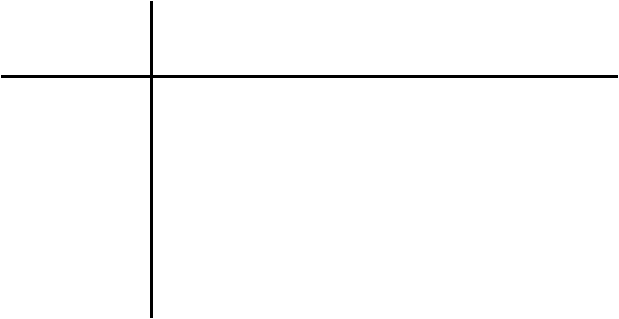
\includegraphics[width=\unitlength,page=1]{figures/dl.pdf}}%
    \put(0.20382337,0.43268764){\color[rgb]{0,0,0}\makebox(0,0)[rb]{\smash{task}}}%
    \put(0.28459882,0.43268764){\color[rgb]{0,0,0}\makebox(0,0)[lb]{\smash{duration on machine}}}%
    \put(0.20382337,0.28459932){\color[rgb]{0,0,0}\makebox(0,0)[rb]{\smash{a}}}%
    \put(0.20382337,0.16343615){\color[rgb]{0,0,0}\makebox(0,0)[rb]{\smash{b}}}%
    \put(0.20382337,0.04227298){\color[rgb]{0,0,0}\makebox(0,0)[rb]{\smash{c}}}%
    \put(0,0){\includegraphics[width=\unitlength,page=2]{figures/dl.pdf}}%
  \end{picture}%
\endgroup%
}
\caption{Flow shop instance with three tasks and two machines\label{fig:fs:ins}}
\end{figure}
\begin{figure}[ht]
\centering
{\def\svgwidth{\linewidth}
%% Creator: Inkscape inkscape 0.91, www.inkscape.org
%% PDF/EPS/PS + LaTeX output extension by Johan Engelen, 2010
%% Accompanies image file 'dl-sol.pdf' (pdf, eps, ps)
%%
%% To include the image in your LaTeX document, write
%%   \input{<filename>.pdf_tex}
%%  instead of
%%   \includegraphics{<filename>.pdf}
%% To scale the image, write
%%   \def\svgwidth{<desired width>}
%%   \input{<filename>.pdf_tex}
%%  instead of
%%   \includegraphics[width=<desired width>]{<filename>.pdf}
%%
%% Images with a different path to the parent latex file can
%% be accessed with the `import' package (which may need to be
%% installed) using
%%   \usepackage{import}
%% in the preamble, and then including the image with
%%   \import{<path to file>}{<filename>.pdf_tex}
%% Alternatively, one can specify
%%   \graphicspath{{<path to file>/}}
%% 
%% For more information, please see info/svg-inkscape on CTAN:
%%   http://tug.ctan.org/tex-archive/info/svg-inkscape
%%
\begingroup%
  \makeatletter%
  \providecommand\color[2][]{%
    \errmessage{(Inkscape) Color is used for the text in Inkscape, but the package 'color.sty' is not loaded}%
    \renewcommand\color[2][]{}%
  }%
  \providecommand\transparent[1]{%
    \errmessage{(Inkscape) Transparency is used (non-zero) for the text in Inkscape, but the package 'transparent.sty' is not loaded}%
    \renewcommand\transparent[1]{}%
  }%
  \providecommand\rotatebox[2]{#2}%
  \ifx\svgwidth\undefined%
    \setlength{\unitlength}{948.00009766bp}%
    \ifx\svgscale\undefined%
      \relax%
    \else%
      \setlength{\unitlength}{\svgscale\unitlength}%
    \fi%
  \else%
    \setlength{\unitlength}{\svgwidth}%
  \fi%
  \global\let\svgwidth\undefined%
  \global\let\svgscale\undefined%
  \makeatother%
  \begin{picture}(1,0.45569621)%
    \put(0.13924056,0.23206748){\color[rgb]{0,0,0}\makebox(0,0)[lb]{\smash{a c b}}}%
    \put(0,0){
\includegraphics[width=\unitlength,page=2]{figures/dl-sol.pdf}}%
    \put(0.1139241,0.18565396){\color[rgb]{0,0,0}\makebox(0,0)[rb]{\smash{1}}}%
    \put(0.1139241,0.14767931){\color[rgb]{0,0,0}\makebox(0,0)[rb]{\smash{2}}}%
    \put(0,0){
\includegraphics[width=\unitlength,page=3]{figures/dl-sol.pdf}}%
    \put(0.1139241,0.41772158){\color[rgb]{0,0,0}\makebox(0,0)[rb]{\smash{machine}}}%
    \put(0.13924056,0.36708866){\color[rgb]{0,0,0}\makebox(0,0)[lb]{\smash{a b c}}}%
    \put(0,0){
\includegraphics[width=\unitlength,page=4]{figures/dl-sol.pdf}}%
    \put(0.1139241,0.32067507){\color[rgb]{0,0,0}\makebox(0,0)[rb]{\smash{1}}}%
    \put(0.1139241,0.28270039){\color[rgb]{0,0,0}\makebox(0,0)[rb]{\smash{2}}}%
    \put(0,0){
\includegraphics[width=\unitlength,page=5]{figures/dl-sol.pdf}}%
    \put(0.13924056,0.41772158){\color[rgb]{0,0,0}\makebox(0,0)[lb]{\smash{solution}}}%
    \put(0,0){
\includegraphics[width=\unitlength,page=6]{figures/dl-sol.pdf}}%
    \put(0.13924056,0.0970464){\color[rgb]{0,0,0}\makebox(0,0)[lb]{\smash{b a c}}}%
    \put(0,0){
\includegraphics[width=\unitlength,page=7]{figures/dl-sol.pdf}}%
    \put(0.1139241,0.0506329){\color[rgb]{0,0,0}\makebox(0,0)[rb]{\smash{1}}}%
    \put(0.1139241,0.01265828){\color[rgb]{0,0,0}\makebox(0,0)[rb]{\smash{2}}}%
    \put(0.5696203,0.23206748){\color[rgb]{0,0,0}\makebox(0,0)[lb]{\smash{c a b}}}%
    \put(0,0){
\includegraphics[width=\unitlength,page=8]{figures/dl-sol.pdf}}%
    \put(0.5696203,0.36708846){\color[rgb]{0,0,0}\makebox(0,0)[lb]{\smash{b c a}}}%
    \put(0,0){
\includegraphics[width=\unitlength,page=9]{figures/dl-sol.pdf}}%
    \put(0.5696203,0.0970463){\color[rgb]{0,0,0}\makebox(0,0)[lb]{\smash{c b a}}}%
    \put(0,0){
\includegraphics[width=\unitlength,page=10]{figures/dl-sol.pdf}}%
  \end{picture}%
\endgroup%
}
\caption{Flow shop solutions for all possible permutations\label{fig:fs:sol}}
\end{figure}
% --------------------------------------------------------------------------------
%
For a more involved example, we consider the flow shop problem.
The flow shop problem creates a schedule for a set of tasks $T$ that have to be consecutively executed on $m$ machines.
%
Each task has to be processed on each machine from $1$ to $m$. 
Different parts of one task are completed on each machine resulting in the completion of the task after execution on all machines is finished.
Before a task can be processed on machine $i$, it has to be finished on machine $i-1$.
The duration of different tasks on the same machine may vary.
A task can only be executed on one machine at a time and
a machine must not be occupied by more than one task at a time.
%
A solution to the problem is a permutation of the tasks and starting times for all tasks on all machines so that no conflicts occur.

Figure~\ref{fig:fs:ins} depicts a possible instance for the flow shop problem.
The three tasks \code{a}, \code{b}, and \code{c} have to be scheduled on two machines.
The colored boxes indicate how long a task has to run on a machine.
Lighter shades of the same color are for the first and darker ones for the second machine.
For example, task \code{a} needs to be processed for~$3$ time units on the first and~$4$ time units on the second machine.

% --------------------------------------------------------------------------------
\lstinputlisting[float=ht,mathescape=true,escapeinside={\#(}{\#)},basicstyle={\ttfamily\small},label={prg:fs:ins},caption={Flow shop instance}]{examples/shop.lp}
% --------------------------------------------------------------------------------
\lstinputlisting[float=ht,literate={\%\%}{}{0},mathescape=true,escapeinside={\#(}{\#)},basicstyle={\ttfamily\small},label={prg:fs:enc},caption={Flow shop encoding}]{examples/flow.lp}
% --------------------------------------------------------------------------------
%
Next, we encode this problem using difference constraints.
We give in Listing~\ref{prg:fs:ins} a straightforward encoding of the instance in Figure~\ref{fig:fs:ins}.
Listing~\ref{prg:fs:enc} depicts the encoding of the flow shop problem.
Following the generate, define, and test methodology of ASP,
we first generate in lines~\ref{prg:fs:perm:begin}--\ref{prg:fs:perm:end} all possible permutations of tasks,
where atoms of form \code{perm(T,U)} encode that task~$T$ has to be executed before task~$U$.
Then, in the following lines~\ref{prg:fs:diff:begin}--\ref{prg:fs:diff:end},
we use difference constraints to calculate the duration of the generated permutation.
%
The difference constraint in Line~\ref{prg:fs:permutation:seq} guarantees that the tasks are executed in the right order.
For example, $\code{(a,1)} - \code{(a,2)} \leq -d$ ensures that task~\code{a} can only be executed on machine~\code{2} if it has finished on machine~\code{1}.
Hence, variable \code{(a,2)} has to be assigned so that it is greater or equal to $\code{(a,1)}+d$ where $d$ is the duration of task \code{a} on machine \code{1}.
Similarly, $\code{(a,1)} - \code{(b,1)} \leq -d$ makes sure that task~\code{b} can only be executed on machine~\code{1} if task~\code{a} has finished on machine~\code{1}.
While the first constraint is a fact (see Line~\ref{prg:fs:permutation:seq:machine}),
the latter is subject to the generated permutation of tasks (see Line~\ref{prg:fs:permutation:seq:task}).
%
The difference constraint in Line~\ref{prg:fs:null} ensures that all time points at which a task is started are greater than zero.
Note that this constraint is in principle redundant
but since sets of difference constraints may have infinitely many solutions
it is good practice to encode relative to a starting point.
Furthermore, note that~\code{0} is actually a variable.
This is a dedicated variable that is always assigned the value 0 and can be used to encode difference constraints with only one variable.

Running encoding and instance with \clingoM{DL} results in the following $6$ solutions
corresponding to the solutions in Figure~\ref{fig:fs:sol}.%
\footnote{Note that in each solution all tasks are executed as early as possible.
  This is due to the guaranteed ASAP assignment as mentioned above.}
One for each possible permutation of tasks:
\marginlabel{%
  To inspect the output, invoke:\\
  \code{\mbox{~}clingo-dl \attach{examples/flow.lp}{flow.lp} \textbackslash\\  
        \mbox{~~~}\attach{examples/shop.lp}{shop.lp.} 0}\\
}
 \begin{lstlisting}[numbers=none]
clingo-dl version 1.0.0
Reading from flow.lp ...
Solving...
Answer: 1
dl((a,1),"1")  dl((a,2),"7") dl((b,1),"0") dl((b,2),"1") 
  dl((c,1),"4") dl((c,2),"11") perm(b,a) perm(a,c)
Answer: 2
dl((a,1),"6") dl((a,2),"16") dl((b,1),"5") dl((b,2),"10") 
  dl((c,1),"0") dl((c,2),"5") perm(b,a) perm(c,b)
Answer: 3
dl((a,1),"0") dl((a,2),"3") dl((b,1),"8") dl((b,2),"13") 
  dl((c,1),"3") dl((c,2),"8") perm(c,b) perm(a,c)
Answer: 4
dl((a,1),"6") dl((a,2),"12") dl((b,1),"0") dl((b,2),"1") 
  dl((c,1),"1") dl((c,2),"7") perm(b,c) perm(c,a)
Answer: 5
dl((a,1),"0") dl((a,2),"3") dl((b,1),"3") dl((b,2),"7") 
  dl((c,1),"4") dl((c,2),"13") perm(b,c) perm(a,b)
Answer: 6
dl((a,1),"5") dl((a,2),"10") dl((b,1),"8") dl((b,2),"14") 
  dl((c,1),"0") dl((c,2),"5") perm(c,a) perm(a,b)
SATISFIABLE

Models       : 6
Calls        : 1
...
\end{lstlisting}
\end{example}

\subsubsection{Advanced Options of \clingoM{DL}}\label{sec:dl:advanced}

In the following, we will consider the two main parameter that may change \clingoM{DL}'s behavior:
\begin{align*}
 \code{--strict}& \text{ : enables strict semantics}\\
 \code{--rdl}& \text{ : variables and constants of the difference constraints have real values} 
\end{align*}

\paragraph{Strict and Non-strict Semantics}

First, let us consider the \emph{strict semantics} option.
In the default configuration, this option is omitted and \clingoM{DL} works with a \emph{non-strict semantics}.
This option changes the logical connection of the difference constraint atom to the difference constraint it represents.
The connections are as follows:
\begin{align*}
 \text{non-strict :}\quad&\code{\&diff\text{ }\{$x$-$y$\}\text{ }<=\text{ }$k$} \quad\Rightarrow\quad x-y\leq k\\
 \text{strict :}\quad&\code{\&diff\text{ }\{$x$-$y$\}\text{ }<=\text{ }$k$}\quad \Leftrightarrow \quad x-y\leq k
\end{align*}

Here, the arrows represent logical implication and equivalence, respectively.
Intuitively, as mentioned above, in the non-strict case, 
if a difference constraint atom holds, the difference constraint has to hold as well,
while no constraint has to be considered by the QF-IDL theory if the respective difference constraint atom is false.
In contrast, strict semantics enforces the negation of the difference constraint to be satisfied if the difference constraint atom is false.
For instance, using the strict semantics, if the difference constraint atom $\code{\&diff\text{ }\{x-y\}\text{ }<=\text{ }-3}$ is false,
the difference constraint $\code{y}-\code{x}\leq 2$ has to hold, which is the negation of $\code{x}-\code{y} \leq -3$.

\begin{example}\label{ex:dl:strict}
We revisit Example~\ref{ex:dl:simple} with strict semantics:
\marginlabel{%
  To inspect the output, invoke:\\
  \code{\mbox{~}clingo-dl \textbackslash\\ 
        \mbox{~~~}\attach{examples/dl1.lp}{dl1.lp} 0 \textbackslash\\
        \mbox{~~~}--strict}
}
\begin{lstlisting}[numbers=none]
clingo-dl version 1.0.0
Reading from dl1.lp
Solving...
Answer: 1
dl(x,"0") dl(y,"0")
Answer: 2
dl(x,"0") dl(y,"3") a
SATISFIABLE

Models       : 2
Calls        : 1
...
\end{lstlisting}
As we can see, the answer set without \code{a} shows an assignment for \code{x} and \code{y},
0 for both of them, since the difference constraint $\code{x}-\code{y}\leq2$ has to be satisfied.

Now, we extend the example slightly by adding the fact that difference constraint $\code{x}-\code{y}\leq -4$ has to be satisfied:
\lstinputlisting{examples/dl2.lp}
Running this example with strict semantics results in the following output:
\marginlabel{%
  To inspect the output, invoke:\\
  \code{\mbox{~}clingo-dl \textbackslash\\ 
        \mbox{~~~}\attach{examples/dl2.lp}{dl2.lp} 0 \textbackslash\\
        \mbox{~~~}--strict}
}
\begin{lstlisting}[numbers=none]
clingo-dl version 1.0.0
Reading from dl2.lp
Solving...
Answer: 1
dl(x,"0") dl(y,"4") a
SATISFIABLE

Models       : 1
Calls        : 1
...
\end{lstlisting}

Only the answer set with \code{a} remains and the assignment of \code{y} changes to 4 
since both $\code{x}-\code{y}\leq -3$ and $\code{x}-\code{y}\leq -4$ have to be fulfilled.
If \code{a} is false, difference constraints $\code{x}-\code{y}\leq -4$ and $\code{y}-\code{x}\leq 2$ would have to be satisfied,
the first due to the fact in Line~2 and the second due to strict semantics and $\code{\&diff\text{ }\{x-y\}\text{ }<=\text{ }-3}$ being false.
Since there does not exist a valid assignment fulfilling those two constraints, there cannot be an answer set with \code{a} being false.

\end{example}

Let us now consider the usefulness of strict and non-strict semantics in different scenarios.
As a rule of thumb, using difference constraint atoms in the head of rules fits the non-strict semantics 
while usage in the body the strict one.

\begin{example}\label{ex:dl:se}
See following example:
\lstinputlisting{examples/dl3.lp}
Running this example with strict semantics results in the following output:
\marginlabel{%
  To inspect the output, invoke:\\
  \code{\mbox{~}clingo-dl \textbackslash\\ 
        \mbox{~~~}\attach{examples/dl3.lp}{dl3.lp} 0 \textbackslash\\
        \mbox{~~~}--strict}
}

\begin{lstlisting}[numbers=none]
clingo-dl version 1.0.0
Reading from examples/dl3.lp
Solving...
Answer: 1
dl(x,"0") dl(y,"4") a
SATISFIABLE

Models       : 1
Calls        : 1
...
\end{lstlisting}

This constitutes the expected result 
where the only possible answer set contains \code{a} since $\code{x}-\code{y}\leq-4$
has to be satisfied, which implies that $\code{x}-\code{y}\leq-3$ is also satisfied,
which in turn derives \code{a}.

However, switching to non-strict semantics produces a different result:
\marginlabel{%
  To inspect the output, invoke:\\
  \code{\mbox{~}clingo-dl \textbackslash\\ 
        \mbox{~~~}\attach{examples/dl3.lp}{dl3.lp} 0}
}

\begin{lstlisting}[numbers=none]
clingo-dl version 1.0.0
Reading from examples/dl3.lp
Solving...
Answer: 1
dl(x,"0") dl(y,"4")
Answer: 2
dl(x,"0") dl(y,"4") a
SATISFIABLE

Models       : 2
Calls        : 1
...
\end{lstlisting}

Now, there are two answer sets instead of one. 
While both assignments fulfill $\code{x}-\code{y}\leq-4$ since it is a fact,
\code{a} is only derived in the second answer set.
Whenever a difference constraint atom exclusively appears in bodies of rules it is called \emph{external}.
This is the case for the difference constraint atom $\code{\&diff\text{ }\{x-y\}\text{ }<=\text{ }-3}$.
The truth value of an external difference constraint atom is determined by the QF-IDL theory and does not have to be derived by any rule.
In other words, every external difference constraint atom creates an implicit choice rule.
If $\code{\&diff\text{ }\{x-y\}\text{ }<=\text{ }-3}$ is chosen to be false, 
its negation $\code{y}-\code{x}\leq 2$ does not have to be satisfied in the non-strict case.
Therefore, it does not contradict $\code{x}-\code{y}\leq -4$ which always has to be satisfied in this example.

\end{example}

\begin{example}
\marginlabel{%
  To inspect the output, invoke:\\
  \code{\mbox{~}clingo-dl \attach{examples/flow.lp}{flow.lp} \textbackslash\\  
        \mbox{~~~}\attach{examples/shop.lp}{shop.lp.} 0\\
        \mbox{~~~}--strict}
}
Similarly, executing Example~\ref{ex:dl:fs} with strict semantics leads to undesired results.
In this case, the program is unsatisfiable.
Consider the following subset of ground rules that order the execution of tasks \code{a}, \code{b} and \code{c} on resource \code{1}:
\begin{lstlisting}[numbers=none].
&diff {(a,1)-(b,1)} <= -3 :- seq((a,1),(b,1),3).
&diff {(b,1)-(c,1)} <= -1 :- seq((b,1),(c,1),1).
&diff {(a,1)-(c,1)} <= -3 :- seq((a,1),(c,1),3).
\end{lstlisting}
For example, in case of execution order \code{a b c}, 
\code{seq((a,1),(b,1),3)} and \code{seq((b,1),(c,1),1)} is true,
but \code{seq((a,1),(c,1),3)} is false.
Though the last sequence is implied, it is not needed to correctly schedule the tasks and would only add a redundant difference constraint.
The non-strict semantics allows this optimization 
by only requiring difference constraints $\code{(a,1)-(b,1)}\leq -3$ and $\code{(b,1)-(c,1)}\leq -1$ to be true (first two rules)
and leaving the truth value of $\code{(a,1)-(c,1)}\leq -3$ open (third rule). 
The strict semantics, however, enforces the negation of $\code{(a,1)-(c,1)}\leq -3$, $\code{(a,1)-(c,1)}\leq 2$, to hold.
This constitutes a conflict with the first two difference constraints and therefore excludes execution order \code{a b c}.
Other possible permutations encounter similar conflicts, ultimately leading to the program being unsatisfiable under strict semantics.
\end{example}

The previous examples illustrate that either \emph{non-strict semantics with difference constraint atoms in the head} or
\emph{strict semantics with difference constraint atoms in the body} is best practice when working with \clingoM{DL}.
Note that this only applies to non-fact difference constraint atoms since facts behave the same way under either semantics.
In practice, non-strict semantics has a performance advantage.
Using it, one only has to monitor difference constraints represented by difference constraint atoms occurring in the logic program.
Strict semantics, on the other hand, has to consider twice the constraints internally, the original constraint and its negation.

Note that it is possible to translate one semantics into the other.
For example, using non-strict semantics with rules of the form 
  \begin{align*}
    \code{\&diff\text{ }\{$x$-$y$\}\text{ }<=\text{ }$k$ :- $L_1$,$\dots$,$L_n$.}
  \end{align*}
can be translated to integrity constraints with strict semantics
  \begin{align*}
    \code{:- not \&diff\text{ }\{$x$-$y$\}\text{ }<=\text{ }$k$, $L_1$,$\dots$,$L_n$.}
  \end{align*}
achieving the same behavior.
Similarly, rules in strict semantics that derive information using difference constraint atoms in the body
  \begin{align*}
    \code{$H$ :- \&diff\text{ }\{$x$-$y$\}\text{ }<=\text{ }$k$, $L_1$,$\dots$,$L_n$.}
  \end{align*}
can be modeled using non-strict semantics by introducing auxiliary variables:
  \begin{align*}
    \code{\{aux\}.}\\
    \code{\&diff\text{ }\{$x$-$y$\}\text{ }<=\text{ }$k$ :- aux.}\\
    \code{$H$ :- aux, $L_1$,$\dots$,$L_n$.}
  \end{align*}
Those are not general translations but rather guiding examples on how either semantics of choice might be used to achieve the same results.
The latter translation shows the advantage of strict semantics for modeling with difference constraints in rule bodies to derive information.
Only one intuitive rule is needed, whereas a choice and an auxiliary atom has to be introduced in the non-strict setting.
In our experience, the performance advantage using non-strict semantics outweighs the modeling inconvenience.

\paragraph{Quantifier-free Real Difference Logic (QF-RDL)}

Whenever option \code{--rdl} is enabled, the domain of variables and constants are real numbers.
In detail, for a difference constraint atom
 \[
    \code{\&diff\text{ }\{$x$-$y$\}\text{ }<=\text{ }$k$}
 \]
 $x$ and $y$ are now real variables and $k$ is a string representation of the real constant.
For example, $\code{x}-\code{y}\leq -3.25$ would be modeled by the difference constraint atom
 \[
    \code{\&diff\text{ }\{x-y\}\text{ }<=\text{ }"-3.25"}
 \]
Note that \clingoM{DL} currently does not support \code{--rdl} and \code{--strict} simultaneously,
because the exact negation of a real difference constraint cannot be automatically calculated.

\subsubsection{Modeling with Difference Constraints}

Our system \clingoM{DL} requires the user to be familiar with the capabilities and limitations of modeling using difference constraints.
While it is, for example, not possible to express inequalities with more then two variables or variables with coefficients unequal one,
a lot of common linear constraints can be easily expressed.
The following table shows rules with commonly used linear constraints in the head and their \clingoM{DL} counterpart.
Here, we consider linear constraints over integers and non-strict semantics.

\begin{center}
\begin{tabular}{l|l}
\textbf{Rule with linear constraint} & \clingoM{DL}\\\hline
\code{$x\leq k$ $\leftarrow$ $L_1$,$\dots$,$L_n$} & \code{\&diff\text{ }\{$x$-0\}\text{ }<=\text{ }$k$ :- $L_1$,$\dots$,$L_n$.}\\
\code{$x<k$ $\leftarrow$ $L_1$,$\dots$,$L_n$}     & \code{\&diff\text{ }\{$x$-0\}\text{ }<=\text{ }V :- V=$k$-1,$L_1$,$\dots$,$L_n$.}\\
\code{$x\geq k$ $\leftarrow$ $L_1$,$\dots$,$L_n$} & \code{\&diff\text{ }\{0-$x$\}\text{ }<=\text{ }$-k$ :- $L_1$,$\dots$,$L_n$.}\\
\code{$x>k$ $\leftarrow$ $L_1$,$\dots$,$L_n$}     & \code{\&diff\text{ }\{0-$x$\}\text{ }<=\text{ }V :- V=$-k$-1,$L_1$,$\dots$,$L_n$.}\\
\code{$x\leq y+k$ $\leftarrow$ $L_1$,$\dots$,$L_n$}   & \code{\&diff\text{ }\{$x$-$y$\}\text{ }<=\text{ }$k$ :- $L_1$,$\dots$,$L_n$.}\\
\code{$x\geq y+k$ $\leftarrow$ $L_1$,$\dots$,$L_n$}   & \code{\&diff\text{ }\{$y$-$x$\}\text{ }<=\text{ }$-k$ :- $L_1$,$\dots$,$L_n$.}
\end{tabular}
\end{center}


\subsection{ASP and Linear Constraints}
\label{sec:linear:constraints}

Similar to \clingoM{DL}, the system \clingoM{LP} integrates the theory of linear constraints into ASP.
%
This theory deals with constraints of the form $w_1x_1+\dots+w_nx_n\leq k$, 
where $k$ is a real-valued constant and $x_i$ and $w_i$ are real-valued variables and coefficients, respectively, for $1\leq i\leq n$. 
%
The syntactic representative of a linear constraint is a linear constraint atom of the form: 
\[
\code{\&sum\text{ }\{$w_1$*$x_1$:$\boldsymbol{L}_1$;\text{ }\dots;\text{ }$w_n$*$x_n$:$\boldsymbol{L}_n$\}\text{ }<=\text{ }$k$} 
\]
%
Here, $w_i$, $k$ and $x_i$ are terms as described in Section~\ref{subsec:lang:gringo} for $1\leq i\leq n$. 
%
In particular, $w_i$ and $k$ are strings of the form \code{"$n.m$"} with $n\in\mathbb{Z}$ and $m\in\mathbb{N}$ representing a real number.
%
If $m=0$ then we may drop the quotes and just write $n$.
%
Terms $x_i$ are internally interpreted as variable names. 
%
$\boldsymbol{L}_i$ are tuples of literals and correspond to conditions as introduced in Section~\ref{subsec:gringo:terms} for $1\leq i\leq n$.
%
An element of a linear constraint atom belongs to the corresponding sum if its condition holds.
%
We may drop a condition if it is a tautology. 
%
Note that \clingoM{LP} supports further relations, viz. \code{>=}, \code{<}, \code{>}, \code{=} and \code{!=}.
%
Linear constraint atoms may occur in heads and bodies of rules. 
%
A formal introduction of \clingoM{LP} is given in \cite{jakaosscscwa17a}.
%
The following description is conform with the \clingoM{LP} system available at \url{https://github.com/potassco/clingoLP}.

In practice, it is often useful to declare the domain of variables when modeling a problem.
%
To describe the domain of a variable 
one could use two linear constraint atoms as follows:  
\begin{align*}
&\code{\&sum\text{ }\{$x$\}\text{ }>=\text{ }$l$}\\
&\code{\&sum\text{ }\{$x$\}\text{ }<=\text{ }$u$}
\end{align*}
where $l$ and $u$ represent reals and $x$ is a variable name. 
%
Alternatively we are allowed to specify the domain of a variable by using the shorthand  
\[
\code{\&dom\text{ }\{$l$\dots$u$\}\text{ }=\text{ }$x$}
\]

While there are often infinitely many solutions for a consistent set of linear constraints, 
one is often interested in optimal solutions. 
%
In \clingoM{LP} an objective function minimizing a set of weighted variables is given by   
\[
 \code{\&minimize\text{ }\{$w_1$*$x_1$:$\boldsymbol{L}_1$;\text{ }\dots;\text{ }$w_n$*$x_n$:$\boldsymbol{L}_n$\}}
\]
where $w_i$ are reals, $x_i$ are variable names and $\boldsymbol{L}_i$ are conditions for $1 \leq i\leq n$. 
%
Analogously, maximize statements are given by using \code{maximize} instead of \code{minimize}. 
%
Given an answer set containing a consistent set of linear constraint atoms, 
the objective function selects an optimal real-valued variable assignment among all valid assignments. 
%
This does not mean that another answer set is going to be excluded due to worse a optimal value. 
%
If there are several optimization statements, then they are accumulated by adding their elements. 
%
Note that domain declarations and optimization statements of \clingoM{LP} are allowed in heads only. 


\subsubsection{Modeling and Solving with \clingoM{LP}}

In the following, we give some examples to illustrate modeling and solving with \clingoM{LP}.

\begin{example}\label{ex:lp:dl}
Let us consider the following program: 
\lstinputlisting{examples/lp1.lp}
%
Note that this program is analogously to the one of Example~\ref{ex:dl:simple}, but using real-valued constant \code{"4.2"}.
%
Calling the system with the example produces following output:
\marginlabel{
  To inspect the output, invoke:\\
  \code{\mbox{~}clingoLP \attach{examples/lp1.lp}{lp1.lp} 0 \textbackslash \\
        --show-lp-solution} \\
}
\begin{lstlisting}[numbers=none]
...
Answer: 1

LP solution: None

Answer: 2
a
LP solution: optimum=0.0
y=4.2 x=0.0
LP solver calls: 1   Time cplex :  0.000322

SATISFIABLE
...
\end{lstlisting}
There are two answer sets, one with the empty answer set and one containing \code{a}. 
%
Since \code{a} was set to false in the first answer set, 
there was no linear constraint to be solved by the underlying linear programming (lp-)solver (here \cplex), 
which is indicated by \code{LP Solution: None}. 
%
The second answer set contains \code{a} only and the lp-solver returns a pair of the optimization value \code{0.0} and assignments $\code{x}\mapsto0$ and $\code{y}\mapsto4.2$. 
%
If we do not specify an optimization function, then the corresponding value amounts to 0.
%
The line \code{LP solver calls: 1   Time cplex :  0.000322} gives the number of calls of the lp-solver and its needed total time in seconds. 
%
Note that the assignments of real-valued variables \code{x} and \code{y} represent just one possible solution 
and the particular assignment depends on the underlying algorithms of the used lp-solver. 
%
For instance, lp-solver \cplex{} always tries to find a solution as close as possible to zero if there is no objective function given. 
\end{example}

\begin{example}\label{ex:lp:extended}
Let us consider the following program that uses the features of conditions, domains and objective functions:
\lstinputlisting{examples/lp2.lp}
The program contains again a choice on \code{a} (Line~1). 
%
The linear constraint of Line 2 is of form $\code{x}-\code{y}\leq-3$ if \code{a} is false 
and of form $\code{x}-\code{y}+42\code{z}\leq-3$ otherwise. 
%
The domain of variables \code{x}, \code{y} and \code{z} is set to the interval $[0,42]\subset\mathbb{R}$ by lines 3-5. 
%
Line 6 specifies that we are interested in assignments of the real-valued variables so that $\code{y}+2\code{z}$ becomes maximal. 
%
Running the example produces following output:
\marginlabel{
  To inspect the output, invoke:\\
  \code{\mbox{~}clingoLP \attach{examples/lp2.lp}{lp2.lp}   0 \textbackslash\\ 
    --show-lp-solution}\\
}
\begin{lstlisting}[numbers=none]
...
Answer: 1

LP solution: optimum=126.00000000000001
z=42.0 y=42.0 x=0.0
LP solver calls: 1   Time lp_solve :  6.329099999996535e-05

Answer: 2
a
LP solution: optimum=43.85714285714286
z=0.9 y=42.0 x=0.0
LP solver calls: 2   Time lp_solve :  0.00010352799999996387

SATISFIABLE
...
\end{lstlisting}
Again we obtain two answer sets, namely $\{\}$ and $\{\code{a}\}$. 
%
In the first answer set variables \code{y} and \code{z} are assigned to the maximal domain value, due to the objective function. 
%
Variable \code{x} is set to 0 to satisfy $\code{x}-\code{y}\leq-3$. 
%
In the second answer set, we have $\code{x}\mapsto0$, $\code{y}\mapsto42$ and $\code{z}\mapsto0.9$ to satisfy $\code{x}-\code{y}+42\code{z}\leq-3$ and 
obtain the optimal value $43.857142857142854$. 
%
\marginlabel{
  To inspect the output, invoke:\\
  \code{\mbox{~}clingoLP \attach{examples/lp2.lp}{lp2.lp} 0 \textbackslash\\ 
        --show-lp-solution \textbackslash\\ 
        \mbox{~~~}--accuracy=3} \\
}
To print the assignment with three digits after the decimal dot run the same program with the additional parameter \code{--accuracy=3}.
%
This leads to the output: 
\begin{lstlisting}[numbers=none]
...
Answer: 2
a
LP solution: optimum=43.85714285714286
z=0.929 x=0.0 y=42.0
LP solver calls: 2   Time lp_solve :  0.00012673600000001617

SATISFIABLE
...
\end{lstlisting}
%Note that during solving the lp-solver may round values to be able to continue. 
\end{example}


\subsubsection{Advanced Options of \clingoM{LP}}

Similar to \clingoM{DL}, we consider in the following some main parameter of \clingoM{LP}: 

\begin{align*}
 &\code{--strict} && \text{ : enables strict semantics (default is non-strict)}\\
 &\code{--lp-solver=cplx}&& \text{ : sets lp-solver \lpsolve{} or \cplex{} (default \code{lp-solver=lps})}\\
 &\code{--ilp}     && \text{ : restricts variables to integer domains (default \code{ilp=0})}  
\end{align*}

\paragraph{Strict and Non-strict Semantics}
Per default \clingoM{LP} uses non-strict semantics, which can be switched to strict semantics. 
%
As in Section~\ref{sec:dl:advanced}, the logical connection of a linear constraint atom and the linear constraint it represents is given by:
\begin{align*}
 \text{non-strict :}\quad&\code{\&sum\text{ }\{$w_1$*$x_1$;\text{ }\dots;\text{ }$w_n$*$x_n$\}\text{ }<=\text{ }$k$} \quad\Rightarrow\quad w_1x_1+\dots+w_nx_n\leq k\\
 \text{strict :}\quad&\code{\&sum\text{ }\{$w_1$*$x_1$;\text{ }\dots;\text{ }$w_n$*$x_n$\}\text{ }<=\text{ }$k$} \quad \Leftrightarrow \quad w_1x+\dots+w_nx_n\leq k
\end{align*}
We recommend to use linear constraint atoms in the head together with non-strict semantics and in the body with strict semantics, 
to avoid unexpected behaviors as explained in the context of difference constraint atoms. 

\paragraph{lp-solver} 
Note that \clingoM{LP} provides two different underlying lp-solvers, namely \lpsolve{} and \cplex{}. 
%
Both lp-solvers need to be installed to run \clingoM{LP}. 

\paragraph{Integer Linear Programming} 
If one is interested in solving linear constraints containing variables over integer domains, 
then this can be easily done by adding \code{--ilp}. 
%
This does only work if the underlying lp-solver supports this option. 



\subsection{ASP and Constraint Programming}\label{sec:constraint}

\subsubsection{ASP and Constraint Programming with \clingcon}
\label{sec:clingcon}

The \clingcon{} system provides a way to integrate constraints over integer variables, into ASP.
Its main focus is on linear constraints, but other constraints such as $distinct$ and $disjoint$ are also supported.
It uses lazy constraint propagation and utilizes lazy variable creation based on the order-encoding to be able to handle huge domains explicitly.
A formal introduction of \clingcon{} is given in \cite{bakaossc16a}.
%
The following description is conform with the $\clingcon\ 5.5.0$ system available at \url{https://github.com/potassco/clingcon}.
%
The following constraints are support by \clingcon.

\paragraph{Domain Constraints} have the form
\code{\&dom\text{ }\{$v_1$;\dots;$v_n$\}\text{ }=\text{ }$x$} where $v_i$ is either a constant expression%
\footnote{A term that can be evaluated to an integer during grounding.}
or of the form $l$..$u$ where $l$ and $u$ are constant expressions defining the lower and upper bound of a range, for $1\leq i\leq n$.
This construct constrains the domain of integer variable $x$ to the union of the given values and ranges.
E.g.~\code{\&dom\text{ }\{$1$..$3$;$5$;$7$..$9$\}\text{ }=\text{ }$x$} constrains $x$ to be in domain $\{1,2,3,5,7,8,9\}$.
Domain constraints are only allowed to occur in the head of rules.

\paragraph{Linear Constraints} have the form
\code{\&sum\text{ }\{$e_1$;\text{ }\dots;\text{ }$e_{n-1}$\}\text{ }$\rhd$\text{ }$e_n$}
where $e_i$ is an expressions, for $1\leq i\leq n$, 
and $\rhd \in \{\code{<=},\code{<},\code{>=},\code{>},\code{=},\code{!=}\}$.
An expressions $e_i$ can be any linear constraint of the form $w_1$*$x_1$ $\circ$ \text{ }\dots $\circ$ \text{ }$w_m$*$x_m$
with $\circ \in \{\code{+}, \code{-}\}$.
The weight $w_j$ is a constant expression that can be omitted if it is equal to $1$.
The term $x_j$ represents a variable, and can be omitted to express a constant in the linear expression.
If the values of the variables $x_j$ satisfy the constraint $e_1+\dots+e_{n-1} \rhd e_{n}$,
for $1\leq j\leq m$, the constraint must be true, and false otherwise.
Linear constraints can occur anywhere in a rule.
E.g.~\code{\&sum\text{ }\{a-3*b;x+y\}\text{ }=\text{ }2*z+3*w} is a constraint according to the definition.

\paragraph{Distinct constraints} have the form
\code{\&distinct\text{ }\{$e_1$;\text{ }\dots;\text{ }$e_n$\}} and constrain the values of all expressions
$e_i$ to be distinct, for $1\leq i\leq n$.
Distinct constraints are only allowed to occur as facts in the logic program.
E.g.~\code{\&distinct\text{ }\{a;3*b;a-b\}} ensures that \code{a}, \code{3*b}, and \code{a-b} all evaluate to different values.

\paragraph{Disjoint constraints} have the form
\code{\&disjoint\text{ }\{$v_1$@$d_1$;\text{ }\dots;\text{ }$v_n$@$d_1$\}} and constrain the values of all variables
$v_i$ and its integer durations $d_i$ to be disjoint, for $1\leq i\leq n$.
This constraint is equivalent to the conjunction of the expressions $(v_i+d_i < v_j) \lor (v_j+d_j < v_i)$ for all $1\leq i \leq j \leq n$.
Distinct constraints are only allowed to occur as facts in the logic program.
The following example encodes a flow shop problem using the distinct constraint.
\lstinputlisting{examples/csp4.lp}


\paragraph{Optimization constraints} have either the form
\code{\&minimize\text{ }\{$e_1$;\text{ }\dots;\text{ }$e_n$\}} or
\code{\&maximize\text{ }\{$e_1$;\text{ }\dots;\text{ }$e_n$\}}
and minimize/maximize the values of all expressions $e_i$,
for $1\leq i\leq n$.
Optimize constraints are only allowed to occur as facts in the logic program.
\begin{example}\label{ex:lp:csp1}
Consider the following optimize constraint:
\lstinputlisting{examples/csp1.lp}
Calling the system with the example produces following output:
\marginlabel{
  To inspect the output, invoke:\\
  \code{\mbox{~}clingcon \attach{examples/csp1.lp}{csp1.lp}} \\
}
\begin{lstlisting}[numbers=none]
...
Answer: 9

Assignment:
a=-3 b=2
Cost: -11
Answer: 10

Assignment:
a=-3 b=3
Cost: -12
SATISFIABLE
...
\end{lstlisting}
\clingcon{} successively produces better answers with respect to the optimize statement.
The last answer produced is the optimal solution to the problem.
\end{example}
It is not recommended to mix Boolean and CSP optimization statements, as the results are implementation defined.

\subsubsection{Modeling and Solving with \clingcon}
In practice, it is often useful to declare the domain of variables when modeling a problem.
%
To describe the domain of a variable 
one could use two linear constraint atoms as follows:  
\begin{align*}
&\code{\&sum\text{ }\{$x$\}\text{ }>=\text{ }$l$}\\
&\code{\&sum\text{ }\{$x$\}\text{ }<=\text{ }$u$}
\end{align*}
where $l$ and $u$ represent reals and $x$ is a variable name. 
%
Alternatively we are allowed to specify the domain of a variable by using the shorthand  
\[
\code{\&dom\text{ }\{$l$..$u$\}\text{ }=\text{ }$x$}
\]

The solutions produced by the system will include each valid assignment to each integer variable that is
used in a ground constraint.
Variables that occur in a constraint (independent of its truth value in the answer set) that are not
restricted by any constraints are automatically restricted by the system to the range $maxint..minint$.
These values can be configured using the options of the \clingcon{} system.

Note that truth value of a constraint is determined from outside the logic program.
This means that constraints that only occur in the body of a rule also become true,
if the values of its variables satisfy the constraint.

\begin{example}\label{ex:lp:csp2}
Let us consider the following program: 
\lstinputlisting{examples/csp2.lp}
Calling the system with the example produces following output:
\marginlabel{
  To inspect the output, invoke:\\
  \code{\mbox{~}clingcon \attach{examples/csp2.lp}{csp2.lp} 0} \\
}
\begin{lstlisting}[numbers=none]
...
Answer: 1

Assignment:
x=0 y=0
Answer: 2

Assignment:
x=0 y=1
Answer: 3

Assignment:
x=1 y=0
Answer: 4

Assignment:
x=1 y=1
Answer: 5
a
Assignment:
x=0 y=1
SATISFIABLE
...
\end{lstlisting}
There are four answer sets where \code{a} is false.
Therefore, all combinations of values from the domains of the variables \code{x} and \code{y} are possible.
The fifth answer contains \code{a},
and the only possible assignment to the integer variables is \code{x=0} and \code{y=1},
as they are constrained by the constraint \code{\&sum\text{ }\{x; -1*y\}\text{ }<\text{ }0}.
%
Since \code{a} was set to false in the first answer set, 
there was no linear constraint to be solved by the underlying constraint solver, 
still an enumeration of all variables occuring in the ground program is done. 
%
\end{example}

\begin{example}\label{ex:lp:csp3}
Now consider an example with a constraint in the body of a rule: 
\lstinputlisting{examples/csp3.lp}
Calling the system with the example produces the following output:
\marginlabel{
  To inspect the output, invoke:\\
  \code{\mbox{~}clingcon \attach{examples/csp3.lp}{csp3.lp} 0} \\
}
\begin{lstlisting}[numbers=none]
...
Answer: 1

Assignment:
x=0 y=0
Answer: 2

Assignment:
x=1 y=0
Answer: 3

Assignment:
x=1 y=1
Answer: 4
a
Assignment:
x=0 y=1
SATISFIABLE
...
\end{lstlisting}
There are again 4 possible combinations for the assignment of the integer variables \code{x} and \code{y}.
The first three answers do not satisfy the constraint \code{\&sum\text{ }\{x; -1*y\}\text{ }<\text{ }0}, and therefore \code{a} is not contained in the answer set.
Given the valuation in the fourth answer,
the constraint is actually satisfied, directly deriving \code{a}.
\end{example}

\subsubsection{Advanced Options of \clingcon}\label{sec:clingcon:advanced}

This is an incomplete list of options to configure \clingcon.
We restricted ourselves to options that drastically influence the search behaviour.

\paragraph{\texttt{--translate-clauses=<n>[,<m>]}} enables translation of linear constraints prior to solving.
Setting \texttt{n} restricts the preprocessor to only translate constraints that can be translated using at most \texttt{n} clauses.
The additional parameter \texttt{m} stops translation to clauses once \texttt{m} clauses have been created.

\paragraph{\texttt{--[no-]literals-only}} ensures that only order literals are created during translation but no clauses are added.

\paragraph{\texttt{--translate-pb=<n>}} enables translation of linear constraints to pseudo Boolean constraints, if less than \texttt{n} order literals are needed per constraint.
\comment{I changed this option, open PR}

\paragraph{\texttt{--translate-distinct=<n>}} forces the translation of $distinct$ constraint to pseudo Boolean constraints, if less than \texttt{n} pseudo Boolean constraints are needed per $distinct$ constraint.

\paragraph{\texttt{--translate-opt=<n>}} enables the translation of the \code{\&minimize}/\code{\&maximize} constraints to clasp internal optimization constraints, if less than \texttt{n} literals are needed for the translation.
Translating optimization statements can be advantageous in combination with \clingo's option \texttt{--opt-strategy=usc} to allow for different optimization strategies.

\paragraph{\texttt{--[no-]add-order-clauses}} adds all binary order clauses needed for the integer variables before solving.

\paragraph{\texttt{--sign-value=<arg>}} influences the strategy which values are assigned first to an integer variable. While \texttt{+}/\texttt{-} tend to assign larger/smaller numbers,
and integer \texttt{n} can be used to steer variable assignment to this value.

\paragraph{\texttt{--min-int=<l>}} and \texttt{--max-int=<u>} sets the default domain of integer variables to $l..u$ if no specific domain is given in the program.

\subsubsection{ASP and Constraint Programming with \gringo}

Grounder \gringo\ features some \textcolor{red}{experimental} means for expressing finite linear constraint satisfaction problems within ASP's modeling language.
The linear constraints are compiled into normal rules following the order encoding \cite{tatakiba09a,bageinscsotawe13a}.
Hence, off-the-shelf ASP solvers like \clasp\ can be used to solve such problems.

CSP constraints in gringo are build over \emph{constraint terms}, which have form
\[\code{$c_1$~\$*~\$$v_1$~\$+~$\cdots$~\$+~$c_n$~\$*~\$$v_n$}\]
where $n>0$, and each $c_i$ (integer factor) and $v_i$ (name of a constraint variable) are terms.
If a factor is one, then the `\code{$c_i$ \$*}' part can be omitted.
Similarly, it is possible to just add a factor in which case the `\code{\$* $v_i$}' part can be omitted.

\emph{Linear constraints} in \gringo\ are syntactically similar to built-in comparison predicates (cf.\ Section~\ref{subsec:gringo:comp})
but relation symbols have to be preceded with a \code{\$} symbol
\[\code{$t_0$~\$$\prec_1$~$\cdots$~\$$\prec_{n}$~$t_n$}\]
where $n>0$, each $\prec_i$ is a comparison predicate, and each $t_i$ is a constraint term.

In addition, there is the global \emph{disjoint constraint}
\[\code{\#disjoint~\{~$\boldsymbol{t}_1$:$c_1$:$\boldsymbol{L}_1$;$\dots$;$\boldsymbol{t}_n$:$c_n$:$\boldsymbol{L}_n$~\}}\]
where $n\geq 0$, $\boldsymbol{t}_i$ and $\boldsymbol{L}_i$ are given as in Section~\ref{subsec:gringo:aggregate},
and each $c_i$ is a constraint term.
%
The idea is that sets of values labeled with the same term(s) must be disjoint.

\begin{example}\label{ex:csp:queens1}
\marginlabel{To compute both answer sets, invoke:\\
  \code{\mbox{~}clingo \attach{examples/queensC.lp}{queensC.lp} \textbackslash\\
         \mbox{~} -c n=30}\\
  or alternatively:\\
  \code{\mbox{~}gringo~\attach{examples/queensC.lp}{queensC.lp} \textbackslash\\
        \mbox{~} -c n=30 | clasp 0}
}
For illustration,
consider the following encoding of the $n$-queens puzzle:
\lstinputlisting{examples/queensC.lp}

The first line fixes the domain of the integer variables
\code{\$queen(1)} to \code{\$queen(n)}.
Line~3 forbids queens on the same columns and the last two lines address queens on the same diagonals.
\end{example}

\begin{example}
The next encoding uses the global \code{\#disjoint} constraint:
%
\marginlabel{To compute both answer sets, invoke:\\
  \code{\mbox{~}clingo \attach{examples/queensCa.lp}{queensCa.lp} \textbackslash\\
         \mbox{~} -c n=300}\\
  or alternatively:\\
  \code{\mbox{~}gringo~\attach{examples/queensCa.lp}{queensCa.lp} \textbackslash\\
        \mbox{~} -c n=300 | clasp 0}
}
%
\lstinputlisting{examples/queensCa.lp}
\end{example}

\begin{note}
The \textcolor{red}{current} implementation of constraints in \gringo\ requires 
that all constraint variables appearing in a program must have finite domains inferable from the grounded program.
Hence, rules like in Line~1 of Example~\ref{ex:csp:queens1} fixing the domain of a constraint variable have to be added for each constraint variable.
\end{note}

\subsubsection{Solving CSPs with \aspartame}
\label{sec:aspartame}

This section is not yet ready for publishing
and will be included in one of the forthcoming editions of this guide.

Information on constraint programming with \aspartame\ can be obtained at the following references.

\begin{itemize}
\item URL
\begin{itemize}
\item \url{http://potassco.org/labs}
\item \url{http://www.cs.uni-potsdam.de/aspartame}
\end{itemize}
\item Literature: \cite{bageinscsotawe13a}
\item Description: \aspartame\ solves finite linear CSPs (in XCSP and \sugar{} format) in ASP
\end{itemize}

%%% Local Variables:
%%% mode: latex
%%% TeX-master: "guide"
%%% End:
